%-------------------------------------------------------------------
% BERNOULLI
%-------------------------------------------------------------------

\section{Bernoulli Experiments} \label{Experiments:bernoulli}

In this section we describe and experiment on two Bernoulli data streams. The first is intended to highlight the comparative advantage of CDDM. The second is intended to be a more ``typical" Bernoulli stream to demonstrate that the comparative advantage doesn't only exist for contrived data streams.

\subsection{Setting}

Each instance consists of a Bernoulli variable, and each label is a Bernoulli variable whose rate depends on the value of the instance:
\begin{align}
  \Pr(x=i) &= \begin{cases}
    1-\gamma & \text{if }x=0 \\
    \gamma & \text{if }x=1.
    \end{cases} \\
  \Pr(y=1|x=i) &= \begin{cases}
    \alpha & \text{if }x=0 \\
    \beta & \text{if }x=1.
    \end{cases}
\end{align}
We will call $\gamma$ the instance rate, $\alpha$ the zero rate, and $\beta$ the one rate. The instance-label joint probability of the data stream may be represented graphically as in Figure \ref{fig:bernoulli}.

We are interested in two kinds of concept drift. First we have feature drift, in which the instance rate changes, but the zero and one rate remain the same.
\begin{equation}
  (\gamma,\alpha,\beta) \Rightarrow (\gamma',\alpha,\beta)
\end{equation}
Second, we have real drift concurrent with virtual drift, in which the zero rate, one rate, and instance rate change.
\begin{equation}
  (\gamma,\alpha,\beta) \Rightarrow (\gamma',\alpha',\beta')
\end{equation}
When a drift detector is triggered by real drift, this is a true positive. However, feature drift does not entail an increase in the reducible error. It follows that a model should not be retrained in the case of feature drift. If a drift detector is triggered by feature drift, this is a false positive.

Our experiments with Bernoulli data streams will consist of 1000 time steps under the original distribution, followed by either a real drift or a feature drift, and then 1000 time steps in the new distribution. If a drift detector is triggered after a real drift, then a count of true positives is incremented. If a detector is triggered before a real drift, or after a virtual drift, then a count of false positives is incremented. If a detector is not triggered after a real drift before the 2000 time steps have completed, then a count of false negatives is incremented. We run 2000 iterations of each data stream. The base learner we use is a na\"{i}ve Bayes. Na\"{i}ve Bayes' are known to be poorly calibrated \cite{calibrating}, so are typically a poor choice to use with CDDM. However, this issue arises due to unrealistic independence assumptions which are not invoked in a one-dimensional instance case such as this.

\subsection{Bernoulli-Hard}

To clearly illustrate the comparative advantage of CDDM in data streams with feature drift, we present a data stream called {\bf Bernoulli-hard}. In this data stream, we have one instance which is hard to predict, and one instance which is easy to predict. Specifically, an instance value of zero has zero noise, and an instance value of one has a noise value of 0.2. The instance rate is uniformly sampled.
\begin{align}
  \alpha &= 0 \\
  \beta &= 0.2 \\
  \gamma &\sim U[0,1]
\end{align}
When virtual drift occurs, the instance rate is reversed. When real drift occurs the one rate is reversed.
\begin{align}
  \alpha' &= 0 \\
  \beta &= 0.8 \\
  \gamma' &= 1 - \gamma
\end{align}
If the initial instance rate is less than 0.5, then after virtual drift we will see an increase in the error rate of the model due to an increase in the rate of ``hard problems". This can lead to false positives for drift detectors which use the error-rate operationalisation (henceforth ``error-rate detectors"). Conversely, when the instance rate is greater than 0.5, when real drift occurs we will see a decrease in the rate of ``hard problems", which will decrease the error rate. This may hide the increase in the error rate due to the real drift itself, and can lead to false negatives. These two scenarios are illustrated in Figure \ref{fig:bernoulli_hard}.

More specifically, the change in error rate due to feature drift will be positive when
\begin{align}
  0 &< \Delta E \\
  &< (1-\gamma)\beta - \gamma \beta \\
  &< \beta-2\gamma\beta \\
  \gamma &< 0.5.
\end{align}
Thus, any instance rate greater than 0.5 may trigger false positives in error-rate detectors. The change in error rate due to real drift is positive when
\begin{align}
  0 &< \Delta E \\
  &< (1-\gamma)(1-\beta) - \gamma\beta \\
  &< 1 - \gamma - \beta \\
  \gamma &< 0.8.
\end{align}
Thus false negatives may occur when the instance rate is above 0.8.

The results of the trials on this data stream are given in Table \ref{tab:bernoulli_hard}. We also plot the true positive, false positive and false negative rates against the instance rate to illustrate the results derived in the previous paragraph. 

\begin{figure}
    \centering
    % 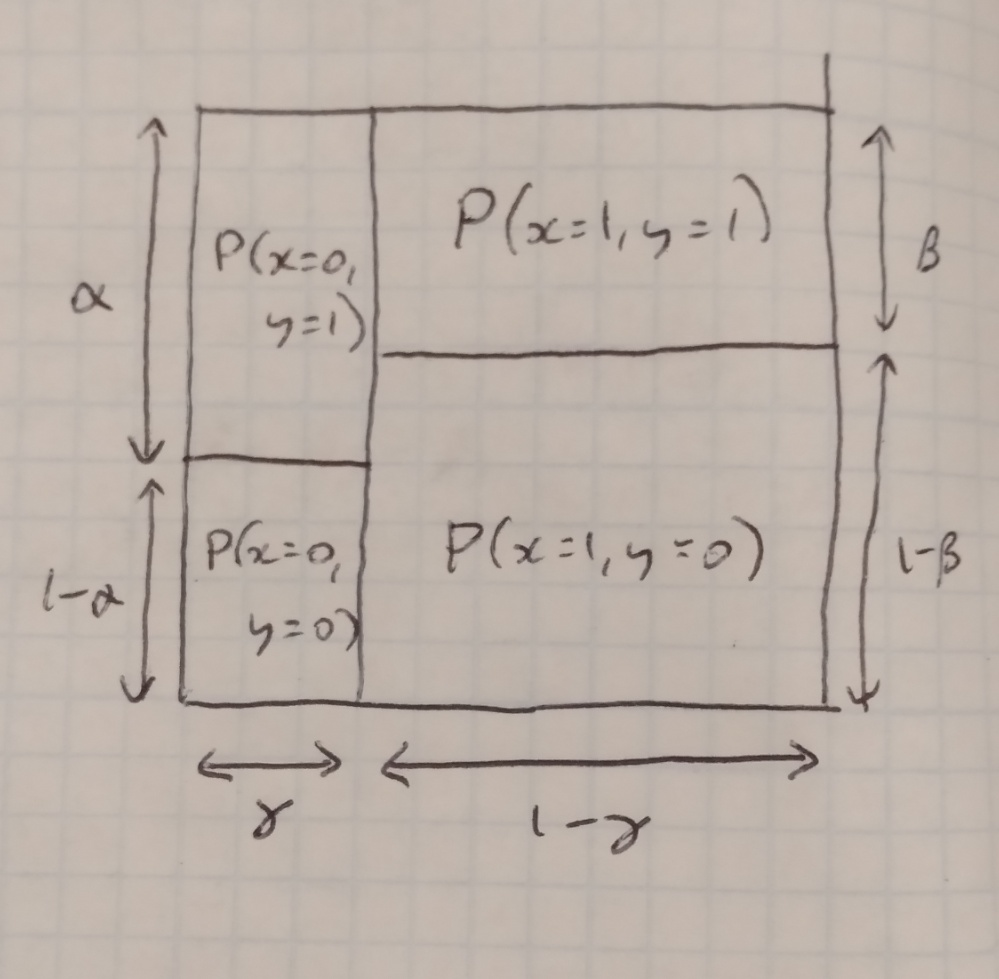
\includegraphics[width=0.5\textwidth]{images/bernoulli.jpg}
    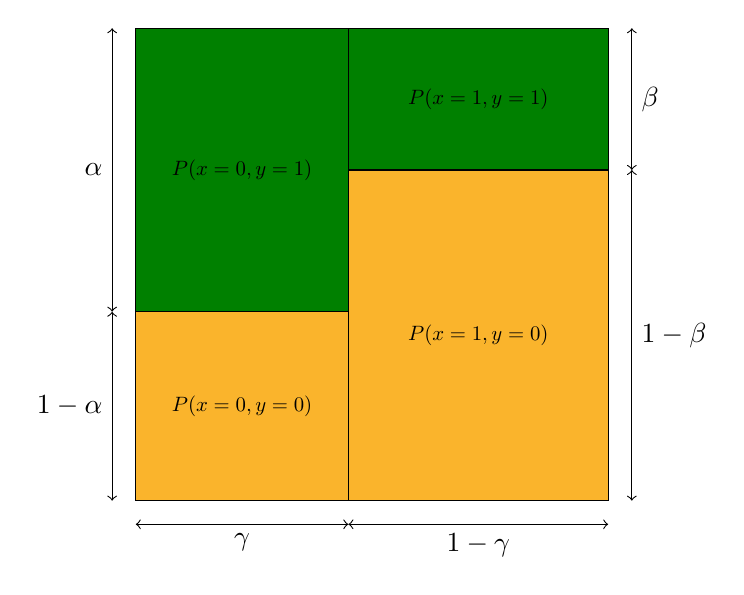
\begin{tikzpicture}[scale=6]
        %--- Arguments ----
        \def \g {0.45} % gamma
        \def \a {0.6} % alpha
        \def \b {0.3} % beta
        \def \zeroColor {Dandelion} % colour of y=0 boxes
        \def \oneColor {Green} % colour of y=1 boxes
        \def \textsep {0.05}
        %--- Rectangles ---
        \draw [fill=\zeroColor] (0,0) rectangle (\g,1-\a);
        \draw [fill=\oneColor] (0,1-\a) rectangle (\g,1);
        \draw [fill=\zeroColor] (\g,0) rectangle (1,1-\b);
        \draw [fill=\oneColor] (\g,1-\b) rectangle (1,1);
        %--- Lines ---
        % alpha
        \draw [<->] (-\textsep, 0) -- (-\textsep, 1-\a);
        \draw [<->] (-\textsep, 1-\a) -- (-\textsep, 1);
        % gamma
        \draw [<->] (0, -\textsep) -- (\g, -\textsep);
        \draw [<->] (\g, -\textsep) -- (1,-\textsep);
        % beta
        \draw [<->] (1+\textsep, 0) -- (1+\textsep, 1-\b);
        \draw [<->] (1+\textsep, 1-\b) -- (1+\textsep, 1);
        %--- Outer labels ---
        % alpha
        \node [left] at (-\textsep, 0.5-\a/2) {$1-\alpha$};
        \node [left] at (-\textsep, 1-\a/2) {$\alpha$};
        % gamma
        \node [below] at (\g/2,-\textsep) {$\gamma$};
        \node [below] at (0.5+\g/2,-\textsep) {$1-\gamma$};
        % beta
        \node [right] at (1+\textsep, 0.5-\b/2) {$1-\beta$};
        \node [right] at (1+\textsep, 1-\b/2) {$\beta$};
        %--- Inner labels ----
        \node [scale=0.75] at (\g/2,0.5-\a/2) {$P(x=0,y=0)$};
        \node [scale=0.75] at (\g/2,1-\a/2) {$P(x=0,y=1)$};
        \node [scale=0.75] at (0.5+\g/2,0.5-\b/2) {$P(x=1,y=0)$};
        \node [scale=0.75] at (0.5+\g/2,1-\b/2) {$P(x=1,y=1)$};
    \end{tikzpicture}
    \caption{Distribution of the Bernoulli data stream.}
    \label{fig:bernoulli}
\end{figure}

\begin{figure}
    \centering
    % 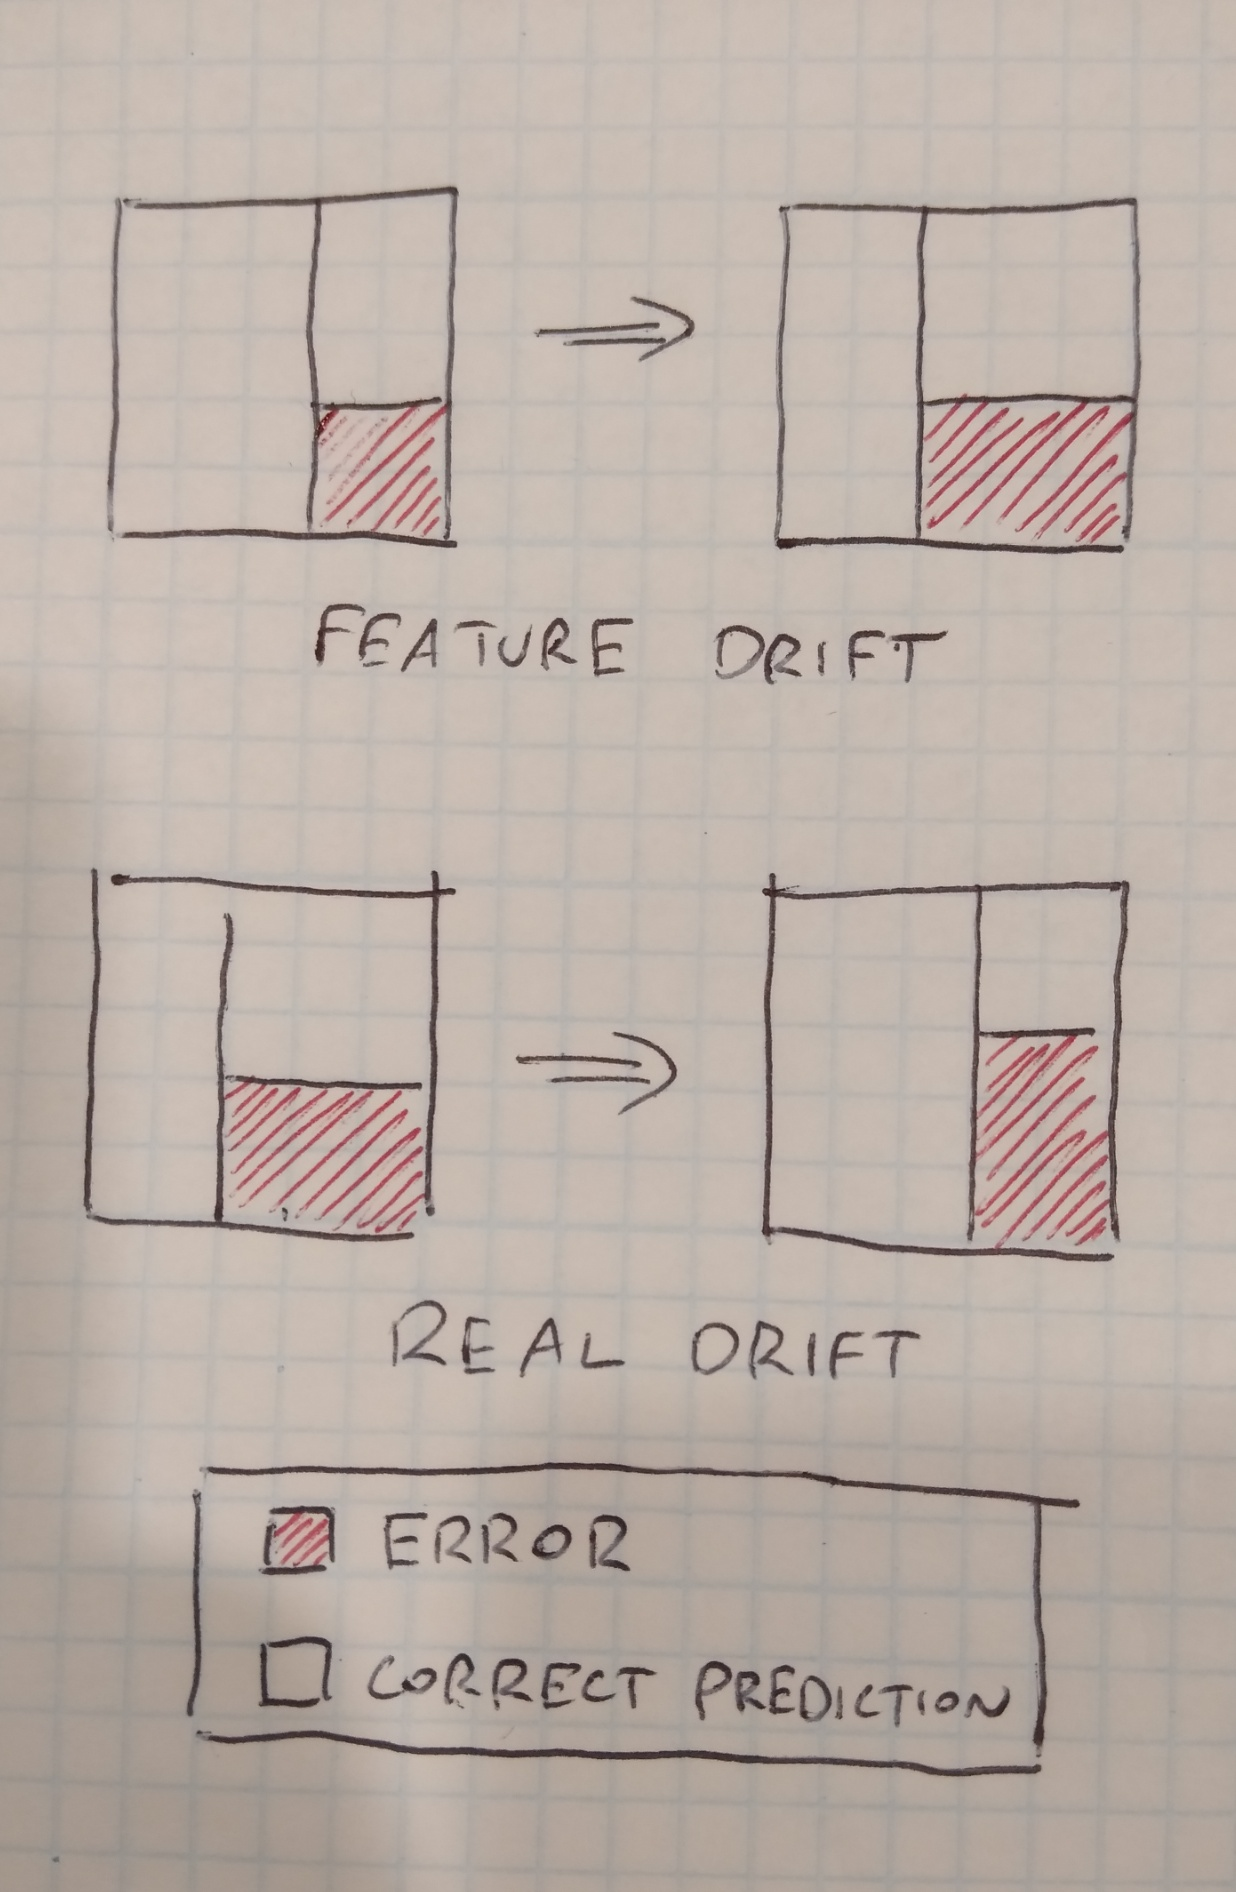
\includegraphics[width=0.5\textwidth]{images/bernoulli_hard.jpg}
    \begin{tikzpicture}[scale=4]
        % --- DEFINITIONS ---
        \def \xSep {2}
        \def \ySep {1.5}
        \def \arrowSep {0.2}
        \def \textSep {0.2}
        \def \gZero {0.25}
        \def \gOne {0.75}
        \def \bZero {0.7}
        \def \bOne {0.3}
        \def \zeroColor {Dandelion} % colour of y=0 boxes
        \def \oneColor {Green} % colour of y=1 boxes
        % \def \zeroColor {Dandelion} % colour of y=0 boxes
        % \def \oneColor {Green} % colour of y=1 boxes
        \newcommand{\bernSqr}[4]{
            % draw a Bernoulli square
            % args:
            %  x value of bottom left
            %  y value of bottom left
            %  gamma
            %  beta
            \draw [fill=\oneColor] (#1,#2) rectangle (#1+#3,#2+1);
            \draw [fill=\zeroColor] (#1+#3,#2) rectangle (#1+1,#2+1-#4);
            \draw [fill=\oneColor] (#1+#3,#2+1-#4) rectangle (#1+1,#2+1);
        }
        % --- SQUARES ---
        \bernSqr{0}{0}{\gZero}{\bZero}
        \bernSqr{\xSep}{0}{\gOne}{\bOne}
        \bernSqr{0}{\ySep}{\gZero}{\bZero}
        \bernSqr{\xSep}{\ySep}{\gOne}{\bZero}
        % --- ARROWS ---
        \draw [ultra thick, ->] (1+\arrowSep,0.5) -- (\xSep-\arrowSep,0.5);
        \draw [ultra thick, ->] (1+\arrowSep,\ySep+0.5) -- (\xSep-\arrowSep,\ySep+0.5);
        % --- TEXT ---
        \node at (0.5+\xSep/2,-\textSep) {Real drift};
        \node at (0.5+\xSep/2,\ySep-\textSep) {Feature drift};
    \end{tikzpicture}
    \caption{Distributional changes in the Bernoulli-hard data stream.}
    \label{fig:bernoulli_hard}
\end{figure}

\subsection{Bernoulli-Typical}

One may object that the previous data stream was tailor-made to showcase CDDM. We demonstrate that this is not the case with another data stream called {\bf Bernoulli-typical} which gives a much more generic picture of false positive and false negative responses from error-rate detectors. In this dataset we do not hand-pick any of the rates. Instead we sample each of them uniformly.
\begin{align}
  \alpha &\sim U[0, 0.5] \\
  \beta &\sim U[0, 0.5] \\
  \gamma &\sim U[0, 1]
\end{align}
The only constraint we place is that after real drift the zero and one rates should increase. This is because most drift detectors deliberately do not detect decreases in the error rate in case it is a result of learning. Allowing decreases in the zero and one rates would thus give CDDM an unfair advantage.
\begin{align}
  \alpha' &\sim U[\alpha, 1] \\
  \beta' &\sim U[\beta, 1] \\
  \gamma' &\sim U[0, 1]
\end{align}

The results of the trials on this data stream are given in Table \ref{tab:bernoulli_hard}.